\documentclass[english,a4,oneside,9pt]{extarticle}
% Author: 
%
%	Oliver Sheridan-Methven, November 2017.
%	
% Description:
%
%	A collection of extremely useful packages 
%	which have been accumulated over a long time,
%	all of which combine to make very nice LaTeX
%	documents. 



\usepackage{adjustbox} % Nice alternative to minipage.
\usepackage{afterpage} % To give the title page its own geometry.
\usepackage{amsmath} % Nice maths symbols.
\usepackage{amssymb} % Nice variable symbols.
\usepackage{array} % Allow for custom column widths in tables.
\usepackage{ltablex} % For long tables spanning multiple pages. % Must be before ARYDSHLN package!
\keepXColumns % Keeps the X column
\usepackage{arydshln} % Dashed lines using \hdashline \cdashline
\usepackage{bbm} % Gives Blackboard fonts.
\usepackage{blindtext} % Generates dummy maths. cf. lipsum.
\usepackage{calc} % Calculates widths of words. 
\usepackage{chngcntr} % Changing counters, e.g. with footnotes.
\usepackage[nostamp]{draftwatermark} % Gives a draft overlay. Use options [nostamp] or [final].
\usepackage{emptypage} % Empty pages have no headers and footers.
\usepackage{enumitem} % Nice listing options in itemize and enumerate.
\usepackage{esdiff} % Gives nice differential operators.
\usepackage{etoolbox} % For defining conditionals. 
\usepackage{fancyhdr} % Nice headers.
\usepackage{float} % Nice figure placement.
\usepackage[T1]{fontenc} % Nice range of text characters and accents.
\usepackage[bottom]{footmisc} % Nice footnote formatting.
\usepackage{graphicx} % Include figures.
\usepackage[notquote]{hanging} % For indenting later lines in a paragraph. USE the 'noquote' option else the `'` is overwritten, and breaks in maths mode!
\usepackage{ifoddpage} % Checks for odd or even page.
\usepackage[geometry]{ifsym} % Useful symbols.
\usepackage{imakeidx} % Makes the index.
\usepackage{indentfirst} % Indents the first paragraph.
\usepackage{letltxmacro} % For defining a nice SQRT symbol.
\usepackage{lipsum} % Useful for adding jargon.
\usepackage{listings} % The listings package for code.
\usepackage{marginnote} % For nice margin notes.
\usepackage{mathtools} % Gives the colon equals symbol.
\usepackage[framed,numbered,autolinebreaks,useliterate]{mcode} % Inports Listings package ideal for MATLAB.
\usepackage[framemethod=tikz]{mdframed} % Gives nices boxed and sidesrules.
\usepackage{multirow} % Nice table cells spanning many rows.
\usepackage{multicol} % If I want to use multiple columns.
\usepackage[numbers, sort&compress]{natbib} % Nice references.
\usepackage{sansmath} % Gives a changing math font. %% Must be before newpxtext/newpxmath ! %%
\usepackage{newpxtext} % Gives Palatino and Helvetica fonts.
\usepackage{newpxmath} % Gives Palatino and Helvetica fonts in maths. 
\usepackage{bm} % Bold math symbols. %% Needs to be loaded after newpxtext/math. %%
\usepackage{nicefrac} % Gives nice fractions for superscripts.
\usepackage{nomencl} % Gives a symbol nomenclature. 
\usepackage[super]{nth} % Gives nice ordinal superscripts, eg 1st, 2nd, etc.
\usepackage{parskip} % Gives nicer indenting.
\usepackage{physics} % Nice partial derivatives and BRAKET notation.
\usepackage{ragged2e} % For nice allignment.
\usepackage{romannum} % Nice typing for roman numerals.
\usepackage{setspace} % Ideal for increasing line spacing. E.g.  \doublespacing
\usepackage{siunitx} % Nice formating of units.
\usepackage{sidenotes} % Nice margin figures and margin tables. 
\usepackage{subcaption} % Side by side figures.
\usepackage[textsize=small]{todonotes} % A nice TODO list. [disable] to supress.
\usepackage{tikz} % Nice diagrams.
\usepackage{titling} % Access title variables. 
\usepackage{titlesec} % Nice section title colouring options.
\usepackage[nottoc]{tocbibind} % Gives nices Table of Contents
\usepackage{xcolor} % This is useful for making greyed table cells, nice for headers. Known preamble placement issues.
\usepackage{xifthen}% Provides \isempty test.
\usepackage{xparse} % Gives \NewDocumentEnvironment which has nice optional argument handling.
\usepackage{xspace} % Gives nice spacing for commands.
%%%% Generally HYPERREF should be imported last. %%%%
\usepackage[colorlinks=true,linkcolor=black,urlcolor=black,citecolor=black,anchorcolor=black]{hyperref} % Colour links.
%%%% Should be loaded after hyperref. %%%%
\usepackage{cleveref} % Gives smart referencing. %% After Hyperref
\usepackage[margin=0pt,textfont=bf, font=small,labelfont=bf,labelsep=endash]{caption} % Caption figures and tables nicely. %% After cleveref.
\usepackage[left=60mm,right=26mm,top=30mm,bottom=29mm, heightrounded, marginparwidth=41mm, marginparsep=8mm, headsep=10mm]{geometry} % Use nice margins. Does give a small change in the default page margins. 

\makeatletter
\if@twoside % commands below work only for twoside option of \documentclass
\newgeometry{left=26mm,right=60mm,top=30mm,bottom=29mm, heightrounded, marginparwidth=41mm, marginparsep=8mm, headsep=10mm}
\fi
\makeatother

% Ensures subsubsections are numbered.
\setcounter{secnumdepth}{3}

% Making an index. 
\makeindex

% Making a nomenclature. 
\makenomenclature
% The column width for any nomenclature. 
\setlength\nomlabelwidth{0.2\linewidth}

% Set the table of content depth to only subsections. 
\setcounter{tocdepth}{2}

% Supressing bad box warnings
%\hbadness=10000 

% Where to search for figures. 
\graphicspath{{figures/}{figures/logos/}}

% Table caption label
%\counterwithin{table}{section}

% Essay-like figure style
%\usepackage{chngcntr} % Set the counter depth
%\counterwithin{figure}{section}
%\captionsetup{ % Set the caption style
%   font=footnotesize,
%   labelfont=bf,
%   singlelinecheck=false,
%}

% Present the references in the order they are used.
\bibliographystyle{unsrtnat}
% Reduce spacing between references. 
\setlength{\bibsep}{0pt plus 0.3ex}

% Listing -> Code in environment labels.
\renewcommand{\lstlistingname}{Code}
\crefname{listing}{code}{codes}
\Crefname{listing}{Code}{Codes}
\lstset{
    numbers=left, 
    basicstyle=\ttfamily\footnotesize,
    frame=single, % adds a frame around the code
    xleftmargin=20.4pt,
    xrightmargin=3.4pt,
    %	numbersep=3mm,
}
\newfloat{lstfloat}{htbp}{lop} % environment for placing lisings in to make them float. 

% Nice paragraph indents.
\setlength{\parindent}{0mm}

% Giving the references the right title.
\renewcommand{\bibname}{References}
\renewcommand{\listfigurename}{List of figures}
\renewcommand{\listtablename}{List of tables}

% Removes most hyphenation.
\tolerance=1
\emergencystretch=\maxdimen
\hyphenpenalty=10000
\hbadness=10000

% To change the spacing in lists:
%\setlist{noitemsep} % or \setlist{noitemsep} to leave space around whole list
% or
\setenumerate{itemsep=-0.2em,topsep=0.5em} % Seems to look nice.

% Custom column widths using C{2cm}, L, R, etc.
\newcolumntype{L}[1]{>{\raggedright\let\newline\\\arraybackslash\hspace{0pt}}m{#1}}
\newcolumntype{C}[1]{>{\centering\let\newline\\\arraybackslash\hspace{0pt}}m{#1}}
\newcolumntype{R}[1]{>{\raggedleft\let\newline\\\arraybackslash\hspace{0pt}}m{#1}}

% Gives a nice column separation in multicolumn mode.
\setlength{\columnsep}{5mm}

% Figure environment for use in multicolumn. To put in captions use \captionof{figure}{content of caption}.
\newenvironment{Figure}
{\par\medskip\noindent\minipage{\linewidth}}
{\endminipage\par\medskip}

% Gives the nice SQRT symbol.
\makeatletter
\let\oldr@@t\r@@t
\def\r@@t#1#2{%
    \setbox0=\hbox{$\oldr@@t#1{#2\,}$}\dimen0=\ht0
    \advance\dimen0-0.2\ht0
    \setbox2=\hbox{\vrule height\ht0 depth -\dimen0}%
    {\box0\lower0.4pt\box2}}
\LetLtxMacro{\oldsqrt}{\sqrt}
\renewcommand*{\sqrt}[2][\ ]{\oldsqrt[#1]{#2}}
\makeatother

% Some common math operators which need their own typesetting.
\DeclareMathOperator{\sign}{sign}
\DeclareMathOperator*{\argmin}{argmin}
\DeclareMathOperator*{\argmax}{argmax}

% Number equations down to the subection level, e.g. 1.2.3 is the third equation in
% subsection 2 of section 1.
%\numberwithin{equation}{section}
\newcommand*\tageq{\refstepcounter{equation}\tag{\theequation}}

% This makes the footnote counter reset in each section.
\counterwithin*{footnote}{section}

% Nice spacing in the first row of a table
\newcommand{\firstrowspacing}{\rule{0pt}{2.6ex}}
% For a more open look in tables.
\setlength\extrarowheight{3pt} 

% Some useful text commands.
\newcommand{\nag}{NAG\textsuperscript{\textregistered}\xspace}
\newcommand{\arm}{Arm\textsuperscript{\textregistered}\xspace}

% For nice headers and footers.
\pagestyle{fancy}
\fancyhf{}
\renewcommand{\headrulewidth}{0pt}
\newlength{\oneinch}
\setlength\oneinch{1in}
\newlength{\innermarginonesided}
\setlength\innermarginonesided{\IfBooleanTF{@twoside}{\evensidemargin+1in}{\paperwidth-\textwidth-\oddsidemargin-1in}}


\definecolor{header1}{RGB}{253,252,204}
\definecolor{header2}{RGB}{204,236,255}
\definecolor{header3}{RGB}{37,141,255}
\definecolor{header4}{RGB}{0,117,246}
\definecolor{header5}{RGB}{0,73,154}
\fancyhead[RE]{%
    \begin{adjustbox}{left, minipage=0.9\paperwidth}
        \hspace*{-0.8\innermarginonesided}
        \begin{tikzpicture}
        \fill[fill=header5, draw=header5, minimum height=8mm, minimum width=16.4cm,anchor=west] (0,-1.4em) rectangle (1.0\linewidth,1.5em);
        \fill[fill=header4, draw=header4, minimum height=8mm, minimum width=16.4cm,anchor=west] (0.7\linewidth,-1.4em) rectangle (\linewidth,1.5em);
        \fill[fill=header3, draw=header3, minimum height=8mm, minimum width=16.4cm,anchor=west] (0.8\linewidth,-1.4em) rectangle (\linewidth,1.5em);
        \fill[fill=header2, draw=header2, minimum height=8mm, minimum width=16.4cm,anchor=west] (0.85\linewidth,-1.4em) rectangle (\linewidth,1.5em);        
        \fill[fill=header1, draw=header1, minimum height=8mm, minimum width=16.4cm,anchor=east] (0.9\linewidth,-1.4em) rectangle (\linewidth,1.5em);
        \end{tikzpicture}\end{adjustbox}}
\fancyhead[LO]{%
    \begin{adjustbox}{right, minipage=0.9\paperwidth}
        \hspace*{0.8\innermarginonesided}
        \begin{tikzpicture}[overlay]
        \fill[fill=header5, draw=header5, minimum height=8mm, minimum width=16.4cm,anchor=east] (0,-1.4em) rectangle (1.0\linewidth,1.5em);
        \fill[fill=header4, draw=header4, minimum height=8mm, minimum width=16.4cm,anchor=east] (0,-1.4em) rectangle (0.3\linewidth,1.5em);
        \fill[fill=header3, draw=header3, minimum height=8mm, minimum width=16.4cm,anchor=east] (0,-1.4em) rectangle (0.2\linewidth,1.5em);
        \fill[fill=header2, draw=header2, minimum height=8mm, minimum width=16.4cm,anchor=east] (0,-1.4em) rectangle (0.15\linewidth,1.5em);        
        \fill[fill=header1, draw=header1, minimum height=8mm, minimum width=16.4cm,anchor=east] (0,-1.4em) rectangle (0.1\linewidth,1.5em);
        \end{tikzpicture}\end{adjustbox}}
\newcommand{\textoverline}[1]{$\overline{\mbox{#1}}$}
% The footers are specified but are not the same margin widths as the headers. 
\fancyfoot[LE]{\hspace*{-0.8\innermarginonesided}\begin{adjustbox}{left, minipage=0.9\paperwidth}
        \raggedright
        \color{cyan}\textoverline{\color{black}\underline{\hphantom{\ }\thepage
                \begin{minipage}[c]{0\linewidth}
                    \rule{0pt}{2.5ex}
                \end{minipage}
                \rule{0.9\linewidth}{0pt}\rule{0pt}{2.0ex}}}
    \end{adjustbox}
}
\fancyfoot[RO]{\hspace*{0.8\innermarginonesided}\begin{adjustbox}{right, minipage=0.9\paperwidth}
        \raggedleft
        \color{cyan}\textoverline{\color{black}\underline{
                \begin{minipage}[c]{0\linewidth}
                    \rule{0pt}{2.5ex}
                \end{minipage}
                \rule{0.9\linewidth}{0pt}\rule{0pt}{2.0ex}\thepage\hphantom{\ }}}
    \end{adjustbox}
}
\fancypagestyle{plain}{%
    \fancyhf{}%
    \renewcommand*{\headrulewidth}{0pt}%
}
\cfoot{}


% Make margin notes small
\renewcommand*{\marginfont}{\noindent \small}
\IfBooleanTF{@twoside}{\reversemarginpar}{}% If I want a wider margin by the binding.
% Ensuring nice justification.
\renewcommand\raggedrightmarginnote{\sloppy}
\renewcommand\raggedleftmarginnote{\sloppy}

% Gives a nice quote environment.
\NewDocumentEnvironment{myquote}{O{}}{%
    \begin{center}
        \begin{minipage}{0.85\linewidth}
            \vspace{1ex}
            \centering \itshape \justifying}
        {%
            \ifthenelse{\isempty{#1}}{}{
                \begin{flushright}%The author/source.
                    \normalfont #1
            \end{flushright}}
            \vspace{1ex}
        \end{minipage}
    \end{center}
}

% Gives a nice siderule environment. e.g. \begin{siderules}
\newmdenv[topline=false,bottomline=false,rightline=false,skipabove=\topsep,skipbelow=\topsep]{siderules}

% For a numbered description. Use inside enumerate, \litem{Something} etc. 
\newcommand\litem[1]{\item{\textbf{\underline{\smash{{#1}}:}}}}

% Nice spacing in lists
%\setlist{listparindent=\parindent,parsep=1ex} 

% This aligns figures in the adjust box environment to the inner margin. For use with "myalignedfigure" (below).
\newcommand{\aligninner}{\ifoddpage \raggedright \else \raggedleft \fi}%

% Gives a nice aligned figure environment, where figures are flush to the inner margin overflowing off the outer margin first. Useful for very wide figures, or set of lots of sub figures. 
\NewDocumentEnvironment{myalignedfigure}{O{1.3} O{htb}}{% fractional_linewidth,  position
    \begin{figure}[#2]
        \checkoddpage
        \edef\whichside{\ifoddpage left\else right\fi}
        \begin{adjustbox}{\whichside, minipage=#1\linewidth}}
        {%
        \end{adjustbox}
    \end{figure}
}

% Gives a nice draft text.
\SetWatermarkScale{1}
\SetWatermarkLightness{0.9}

% The oxford comma from cref for multiple citations. 
\newcommand{\creflastconjunction}{, and\nobreakspace}

% Define the dummy sentence, an ancient palindrome.
\def\sator{Sator Arepo tenet opera rotas.\xspace}

% A command to print the sentence repeatedly.
% Argument #1 is the number of times to repeat it.
\newcount\loopcounter
\def\dummysentences#1{%
    \loopcounter = #1
    \loop
    \sator\ %
    \advance\loopcounter by -1
    \ifnum\loopcounter > 0
    \repeat%
}

% Oxford blue
\definecolor{oxfordblue}{RGB}{0, 33, 71}

% Ensuring side boxes have shadows. 
\usetikzlibrary{shadows} % For shadowed boxes.
\tikzset{every shadow/.style={opacity=1}} % Shadows given full opacity. 

% Temporary environment for the InFoMM side bubble. 
\NewDocumentEnvironment{mysidenote}{}{% verticle offset
    \noindent
    \begin{minipage}[t]{\linewidth}		\begin{mdframed}[roundcorner=5pt, linecolor=oxfordblue, linewidth=2pt, backgroundcolor=yellow!40, shadow=true,shadowcolor=black,shadowsize=6pt]\raggedright
        }
        {
        \end{mdframed}
    \end{minipage}
}

% The final command for an InFoMM margin bubble. 
\newcommand{\infommmarginnote}[2][0mm]{\marginnote{\large\sffamily{}\sansmath\begin{mysidenote}{#2}\end{mysidenote}}[{#1}]}

% Useful for drawing a page border. 
\usetikzlibrary{calc}

% Enable blind maths. 
\blindmathtrue

%InFoMM glossary
\NewDocumentEnvironment{infommitemize}{}{% verticle offset
    \noindent
    \begin{itemize}[label={\color{cyan}{$\blacksquare$}}]
    }
    {%
    \end{itemize}
}

\newcommand{\coverimage}[1][cover_image]{
    \newcommand{\thecoverimage}{#1}
}

% Nice colouring of section titles
\titleformat{\section}[block]
{\color{oxfordblue}\normalfont\fontsize{16}{20}\selectfont\bfseries}
{\thesection.}{1em}{}
%{\color{blue}\thesection}{1em}{\thesection.\hspace{1ex}}
\titleformat{\subsection}
{\color{cyan}\normalfont\Large\bfseries}
{\thesection.}{1em}{}
\titleformat{\subsubsection}
{\color{cyan}\normalfont\Large\bfseries}
{\thesection.}{1em}{}

% Shorten the spacing after section headings
\titlespacing\section{0pt}{12pt plus 4pt minus 2pt}{0pt plus 2pt minus 2pt}
\titlespacing\subsection{0pt}{12pt plus 4pt minus 2pt}{0pt plus 2pt minus 2pt}
\titlespacing\subsubsection{0pt}{12pt plus 4pt minus 2pt}{0pt plus 2pt minus 2pt}



% Remove section numbers in TOC. 
%\makeatletter
%\let\latexl@section\l@section
%\def\l@section#1#2{\begingroup\let\numberline\@gobble\latexl@section{#1}{#2}\endgroup}
%\makeatother
% Remove subsection numbers in TOC. 
\makeatletter
\let\latexl@subsection\l@subsection
\def\l@subsection#1#2{\begingroup\let\numberline\@gobble\latexl@subsection{\quad#1}{#2}\endgroup}
\makeatother


\newtoggle{TWOSIDED}
\togglefalse{TWOSIDED}
\makeatletter
\if@twoside % commands below work only for twoside option of \documentclass
\toggletrue{TWOSIDED}
\fi
\makeatother


\title{User Cancellation Modelling:
\\on Clustering of Customer Behaviours}
\author{Victor (Sheng) Wang}
\coverimage[cover_image] % Specify your own image using [].

\begin{document}

% The cover page is a designed to look best on A4 and is designed to be a
% "What you see is what you get".
\thispagestyle{empty} % 'gobble' pagestyle throws issues with nomencl package. 
\afterpage{
%\pagestyle{empty}
\newgeometry{left = 20mm, right = 20mm, top = 15mm, bottom = 10mm}

\newgeometry{left = 20mm, right = 20mm, top = 30mm, bottom = 30mm}
\pagestyle{empty}
\begin{tikzpicture}[remember picture, overlay]
\draw [line width=2mm, oxfordblue]
($ (current page.south west) + (8mm, 8mm) $)
rectangle
($ (current page.north east) + (-8mm, -8mm)$);
\node[anchor=north west, xshift=10mm, yshift=-10mm] at (current page.north west) {
\includegraphics[width=0.3\linewidth]{epsrc_logo}};
\node[anchor=north east, xshift=-10mm, yshift=-10mm] at (current page.north east) {
\includegraphics[width=0.3\linewidth]{infomm_logo_blue}};
\node[anchor=south west, xshift=10mm, yshift=10mm] at (current page.south west) {
\includegraphics[width=0.3\linewidth]{oxford_logo_blue_long}};
\node[anchor=south east, xshift=-10mm, yshift=10mm] at (current page.south east) {
\includegraphics[width=0.4\linewidth]{whizz_logo_long}};
\end{tikzpicture}

\begin{center}
\vfill
{\fontsize{25}{28}\selectfont\color{oxfordblue}\textbf{EPSRC Centre for Doctoral Training in Industrially Focused Mathematical Modelling}}
\vfill
\begin{figure}[h]
\centering
\includegraphics[width=0.7\linewidth]{\thecoverimage}
\end{figure}
\vfill
{\fontsize{25}{28}\selectfont\color{oxfordblue}\textbf{\thetitle}}\\
\vfill
{\fontsize{20}{25}\selectfont\color{oxfordblue}\color{oxfordblue}\textbf{\theauthor}}
\vfill
\end{center}
\restoregeometry
}
\clearpage
	
% Table of contents page.
\afterpage{
	\titleformat{\section}
	{\color{oxfordblue}\normalfont\fontsize{16}{20}\selectfont\bfseries}
	{\color{black}\thesection}{1em}{}
\pagestyle{empty}
%\newgeometry{left=110mm,right=20mm,top=30mm,bottom=29mm, heightrounded, marginparwidth=100mm, marginparsep=5mm}
%\IfBooleanTF{@twoside}{\reversemarginpar}{}
\iftoggle{TWOSIDED}{
\newgeometry{right=110mm,left=20mm,top=30mm,bottom=29mm, heightrounded, marginparwidth=100mm, marginparsep=5mm}
}{
\newgeometry{left=110mm,right=20mm,top=30mm,bottom=29mm, heightrounded, marginparwidth=100mm, marginparsep=5mm}
\reversemarginpar
}
\noindent
\doublespacing
\begin{minipage}[t]{\linewidth}
\tableofcontents
\end{minipage} \\
\marginpar{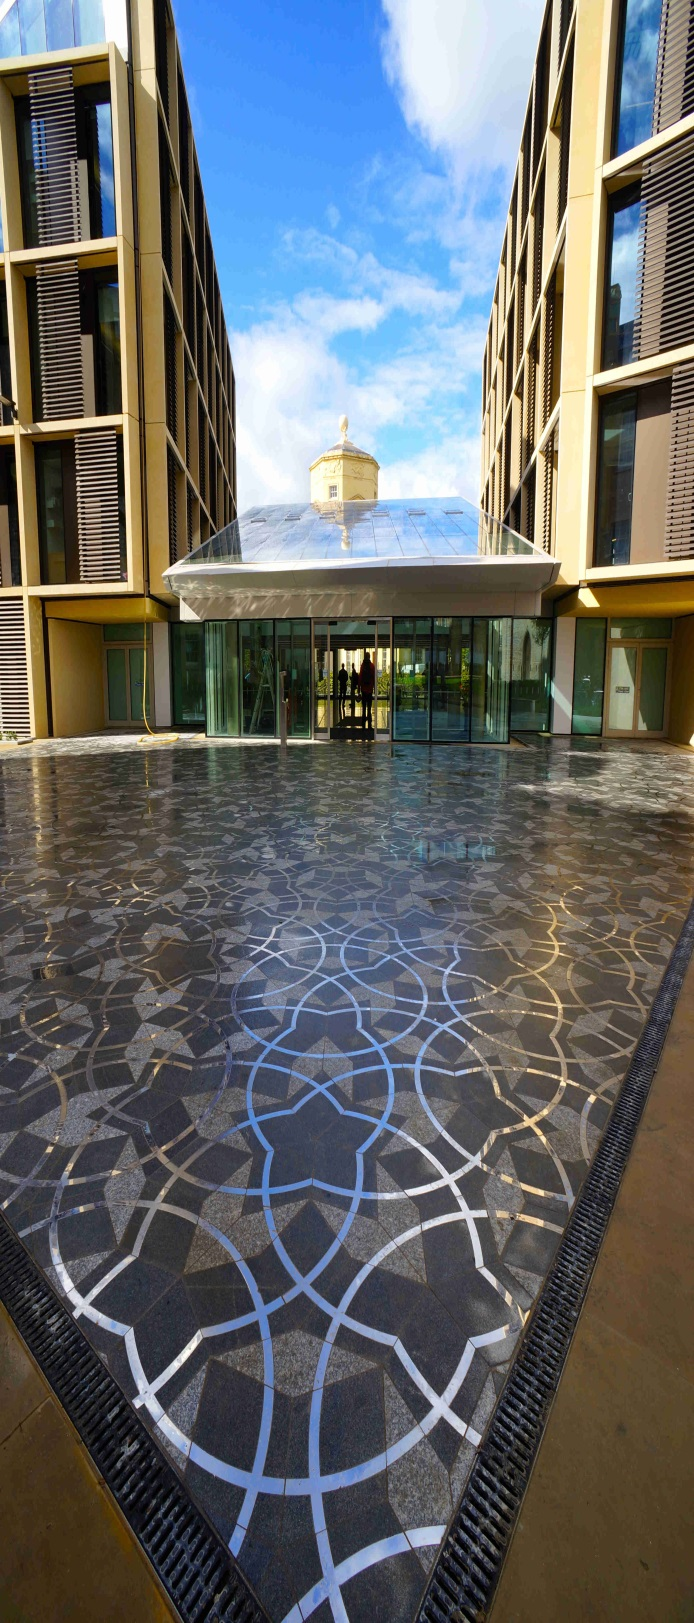
\includegraphics[width=\linewidth]{andrew_wiles_building}}
\clearpage
}
\iftoggle{TWOSIDED}{}{\reversemarginpar}
\cleardoublepage % Double page as page numbering starts at 1.
\setcounter{section}{0}
\pagenumbering{arabic}


% For proof reading
%\doublespacing

\section{Introduction}
\subsection*{Motivation and Goal}
\addcontentsline{toc}{subsection}{Motivation and Goal}

\infommmarginnote[10em]{Churn prediction helps the business to detect customers who are likely to cancel a subscription.}

Retained customers in general create higher revenues than new customers do, and making a sell to a new customer can cost up to 5 times more than encouraging a customer to stay, depending on the business. Therefore, many companies form a Customer Relationship Management (CRM) team with a focus on customer retention strategies. A crucial step is then to identify high risk customers who are intending to discontinue their usage of the services. This assessment is better known as \textit{churn prediction}.

Our project aims to perform the churn prediction task based on making probabilistic clustering assignments of customers' behaviours, and formulate the sequential processes into a scalable pipeline which can be easily reused, updated and extended for many applications. In particular, we apply the pipeline to analyse pupil subscribers' data for Whizz Education (referred to as ``Whizz''). Whizz provides an online virtual tutorial service, Math-Whizz, which pupils can access by purchasing monthly subscriptions. At the end of each subscription, pupils can make the choice to either cancel or do nothing and thereby start a new 1-month subscription.

\subsection*{Train and Prediction Workflow}
\addcontentsline{toc}{subsection}{Train and Prediction Workflow}

Whizz can use the 2-step workflow proposed in \Cref{fig:workflow} to predict pupils' probability of churn, or churn risk, which provides the downstream CRM team with target subscribers to apply retention strategies more efficiently.

\begin{figure}[htb]
\centering
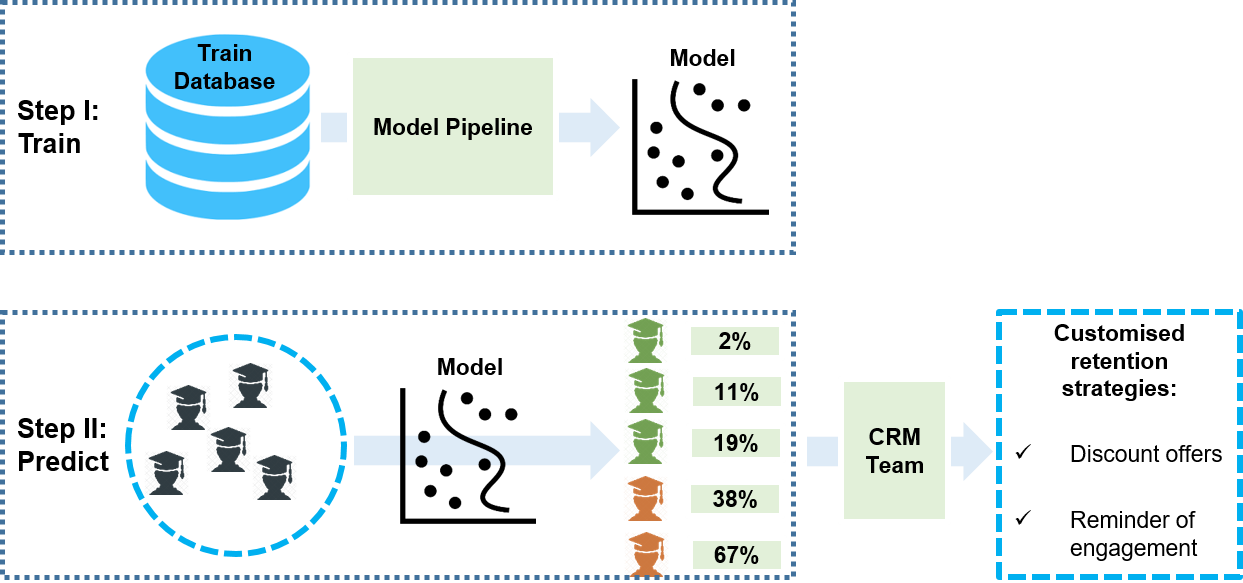
\includegraphics[width=\linewidth]{PredictionWorkflow.png}
\caption{Train and prediction workflow, and its downstream process.}
\label{fig:workflow}
\end{figure} 

\subsection*{Glossary of Terms}
\addcontentsline{toc}{subsection}{Glossary of Terms}

\begin{infommitemize}
	\litem{Clustering} The task of grouping a set of objects in such a way that objects in the same group (called a cluster) are more similar to each other than to those in other groups.
	\litem{Mixture model} A probabilistic model for representing the presence of a mixture of subpopulations within an overall population.
	\litem{Distribution} A mathematical function that provides the probability of occurrence of different possible values of a variable.
	\litem{Markov chain} A model of random event (called a state) that happens over time. The probability of each event depends only on the previous event (Markov property).
\end{infommitemize}

\section{A Generative Process for Customer Behaviours}

Customers' behaviour evolves over time as they respond to business offering and adjust to their own needs. We employ a Markov chain to describe the generative process of customers' behaviours. In addition, we use a mixture model to find Markov states, each of which defines a partition of the behaviours within a single time interval. Splitting pupils' behaviours into monthly time periods is a reasonable representation of the business setting at Whizz. Pupils subscribe to Whizz products on a 1-month contract, and can choose to cancel at the end of current subscription, otherwise a renewal will be made by default.

\subsection*{Customer Journey}
\addcontentsline{toc}{subsection}{Customer Journey}

\infommmarginnote[10em]{Customer month is a time period between the start and the end of a monthly subscription.}

Customer journeys reflect the dynamics of their monthly-behaviours over time. There is inconsistency present in journeys of different customers. The inconsistency refers to the problem that the time intervals for different customers being active in the services are not aligned, so that their behaviours are not comparable. To resolve the inconsistency, we align and aggregate customers' behaviours by switching the reference from calendar month to customer month. This is illustrated by an example in \Cref{fig:customerMonth}.

\begin{figure}[htb]
\centering
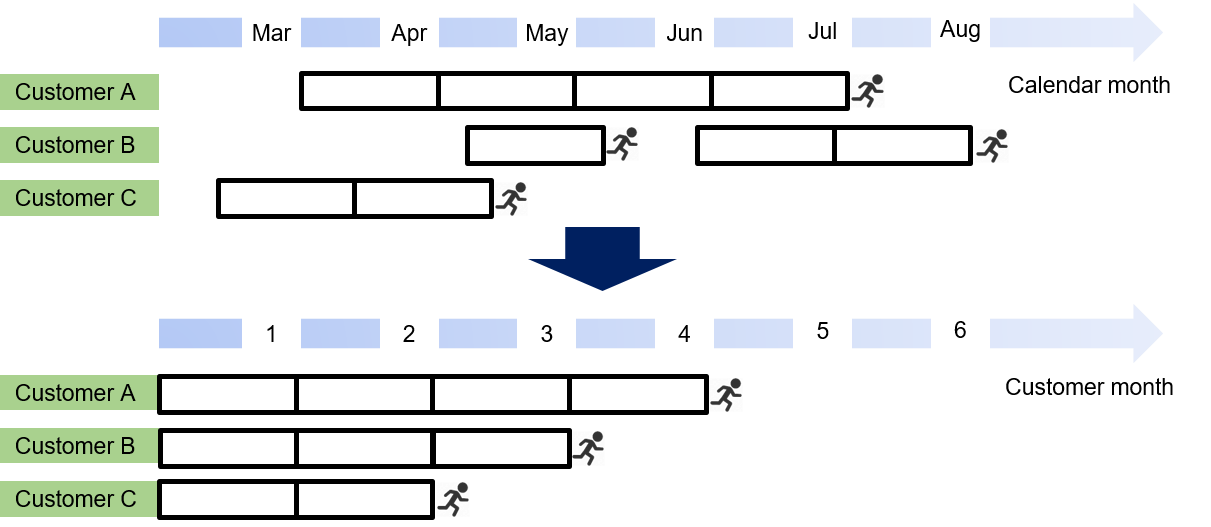
\includegraphics[scale=.6]{CustomerMonth.png}
\caption{Change reference from calendar month to customer month. Customer A, B and C have very different journeys in the sense of subscription start and end dates. Each block represents customer's monthly behaviours. Under calendar month reference, we have to choose studying months from March to August to cover all activities. This choice results in irregular temporal distribution of missing information for all 3 customers. After changing the reference to customer month, behaviours are aligned by customer month and therefore comparable. Moreover, the missing information only occurs after the customer churns. It can also handle discontinuous subscriptions like the case of customer B.}
\label{fig:customerMonth}
\end{figure} 

\infommmarginnote[10em]{An observation is generated as: \\state $\rightarrow$ cluster $\rightarrow$ behaviour.}

\vspace*{-5mm}

\subsection*{Behaviour, Cluster and State}
\addcontentsline{toc}{subsection}{Behaviour, Cluster and State}

We assume that customers with intentions to churn exhibit different behaviours than others do. Behaviours are different distributionally, and generated from a finite number of states. Then the behaviour dynamics of each customer results from a chain of states over time. This formulates into a discrete-time Markov chain with states \textit{transiting} over time, where each state \textit{emits} distinguishable behaviour distribution. An example is given in \Cref{fig:markov}. In brief, a Markov chain is a random process characterised by transition and emission probabilities.

\begin{figure}[htb]
\centering
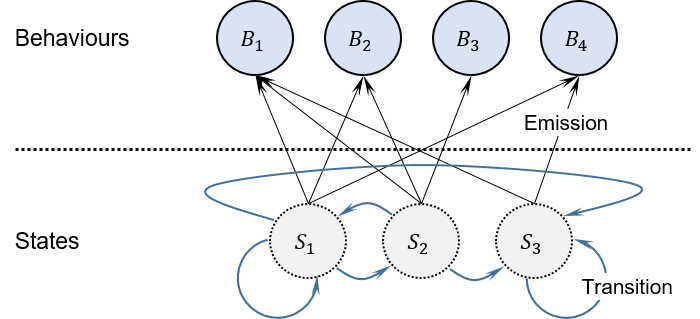
\includegraphics[scale=.7]{Markov.png}
\caption{Behaviours emitted from Markov states. States $S_1$, $S_2$ and $S_3$ generate differently distributed behaviours. For example, $S_1$ generates $\{B_1, B_2, B_4\}$ while $S_3$ produces $\{ B_1, B_4\}$.
Even if the two states can generate the same set of behaviours, the emission probabilities can be different, thus resulting in different behaviour distributions. States transit between each other over time randomly.}
\label{fig:markov}
\end{figure}

The distribution of the emitted behaviours from a state is assumed to be a mixture of component distributions such as uniform, Gaussian, etc. Each component represents a cluster. Therefore, the sequence of observed behaviours are generated in the following way:
\vspace*{-2mm}
\begin{enumerate}
\item At each time step, the system generates a state according to the state-to-state transition.
\vspace*{-1mm}
\item Once the state has been generated, the system generates a cluster according to the state-to-cluster emission probability.
\vspace*{-1mm}
\item Once the cluster has been determined, a behaviour observation is produced probabilistically according to the cluster-parametrised distribution.
\end{enumerate}

\section{Probabilistic Clustering Using Mixture Model}

\infommmarginnote[10em]{A Dirichlet Process Mixture is Bayesian and can infer the number of clusters from data.}

A critical step of the state-cluster-observation Markov chain is the mixture model that describes the probabilistic assignment of observations to clusters. We choose specifically the \textit{Dirichlet Process Mixture} setting which has two important features:
\begin{enumerate}
\item It is Bayesian and treats component parameters as random variables, of which posterior distributions will be updated from a prior as observed data coming in. 
\item The Dirichlet process (DP) is used as a nonparametric prior so that the number of clusters is random and grows as new data are observed.
\end{enumerate}
The benefits of this model choice are massive. Unlike a frequentist's viewpoint, where the observed data as infinitely available as independent replicates like frequentists, here it can be updated with new data as this comes in. Moreover, it infers the number of clusters from observed data and opens the opportunities of finding new clusters as more data are observed.

\section{Modelling Pipeline}

\subsection*{Scope of Data and Features}
\addcontentsline{toc}{subsection}{Scope of Data and Features}

Whizz stores and maintains data generated from business activities in a database consisting of several relational tables. The most relevant tables we use are listed in \Cref{tab:dataTable}. %The study period is from January 1st, 2014 to April 20th, 2018. The number of records within this study period in each data table is also indicated.

\begin{table}[!h]
\centering
\footnotesize
\begin{tabular}{l|p{6cm}|c}
\hline
\textbf{Data Table} & \textbf{Description}  & \textbf{Number of Records} \\
\hline
Account Information &
Pupils' ID and personal information such as date-of-birth. & 2,672 \\
\hline
Subscription history &
Start date and end date of each new subscription or renewed associated with each pupil.  & 17,861 \\
\hline
Lesson history &
Details of each visit activity for each pupil during his subscription period. The visit activity includes the date of visit, time spent, score achieved, lesson outcome, etc. & 450,548 \\
\hline
\end{tabular}
\caption{Description of data tables. The number of records within the study period 2014-01-01 $\sim$ 2018-04-20 in each data table is also indicated.}
\label{tab:dataTable}
\end{table}

A \textit{feature} is an individual measurable property of a behaviour being observed, and choosing informative features is crucial for effective clustering. For example, to measure how often the pupil uses Whizz online tutorial, we can define the time spent or number of visits within a month as the feature. For each customer, we define a collection of features to capture his behaviours of usage, progress, etc. within a customer month.

\subsection*{Modelling Pipeline}
\addcontentsline{toc}{subsection}{Modelling Pipeline}

We summarise the processes of our modelling framework as a pipeline displayed in \Cref{tab:pipeline}. We will apply this pipeline to build a churn prediction model for Whizz.

\begin{figure}[htb]
\marginnote{
    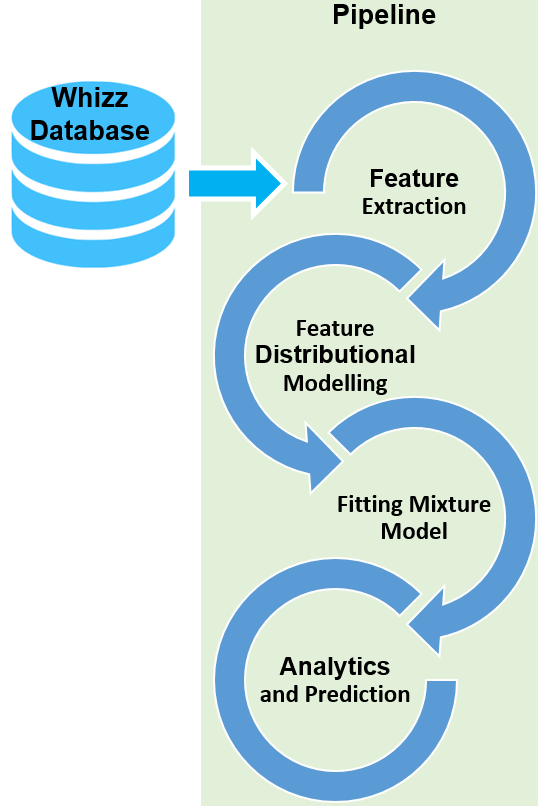
\includegraphics[width=\linewidth]{Pipeline}
    \captionof{figure}{Modelling Pipeline.}
    \label{fig:pipeline}}
\centering
\end{figure}

\begin{table}[htb]
\vspace*{-5mm}
\centering
\footnotesize
\begin{tabular}{c|p{5.5cm}|p{3cm}|p{2.5cm}}
\hline
\textbf{No.} & \textbf{Process} & \textbf{Input} & \textbf{Output} \\
\hline
1 &
\textbf{Feature extraction}: extract informative feature data from historical records of pupils' activity, and represent them in the suitable data structure that can be fed into the behavioral model.&
Raw data from Whizz database that records pupils' ID, subscription history, activity history, etc. & 
Feature data. \\
\hline
2 &
\textbf{Feature distributional modelling}: choose the most suitable distributions for each feature to fit. Independent features can be modelled separately, while correlated features shall be modelled as a part of a multivariate distribution. &
Feature data. & 
Distributional form for each feature. \\
\hline
3.1 &
\textbf{Fitting mixture model}: by assuming behaviours are generated from a Dirichlet process mixtures, make inference on parameters based on observed features.&
Feature data, feature distributional form, mixture model.& 
A collection of clusters. \\
\hline
3.2 &
\textbf{Fitting Markov chain}: use the identified clusters as well as churn outcome information to define states; uncover their transition probabilities. &
Identified probabilistic clusters with distributional form; churn outcome. & 
A finite set of states and state-to-state transition probabilities. \\
\hline
4.1 &
\textbf{Analytics on behaviours}: study the properties of pupils' behaviours such as the temporal transition probabilities, how each feature impact the level of churn risk, etc. &
States, transition, cluster churn rate etc. & 
Temporal state transition analysis, feature analysis, etc. \\
\hline
4.2 &
\textbf{Prediction on new pupils}: predict the level of churn risk for new pupils based on their behaviours with the observation-cluster-state probabilistic assignment trained from previous steps. &
States, clusters, cluster-state assignment. & 
State assignment for new pupils as well as their associated level of churn risk. \\
\hline
\end{tabular}
\caption{Modelling pipeline showing processes in sequence, along with the input and output of each modular process. The last two process 4.1 and 4.2 are independent from each other and are performed for different purposes.}
\label{tab:pipeline}
\end{table}

\section{Clustering Analytics}

We assume that most features can be described by a mixture of multivariate Gaussians. For those whose empirical distribution deviates too much from a Gaussian, we verify their independence from other features and model them as a general mixture of any suitable simple distribution such as uniform, exponential, etc. Examples are shown in \Cref{fig:fitIndependentFeature}.

\begin{figure}[!h]
\centering
\vspace*{-3mm}
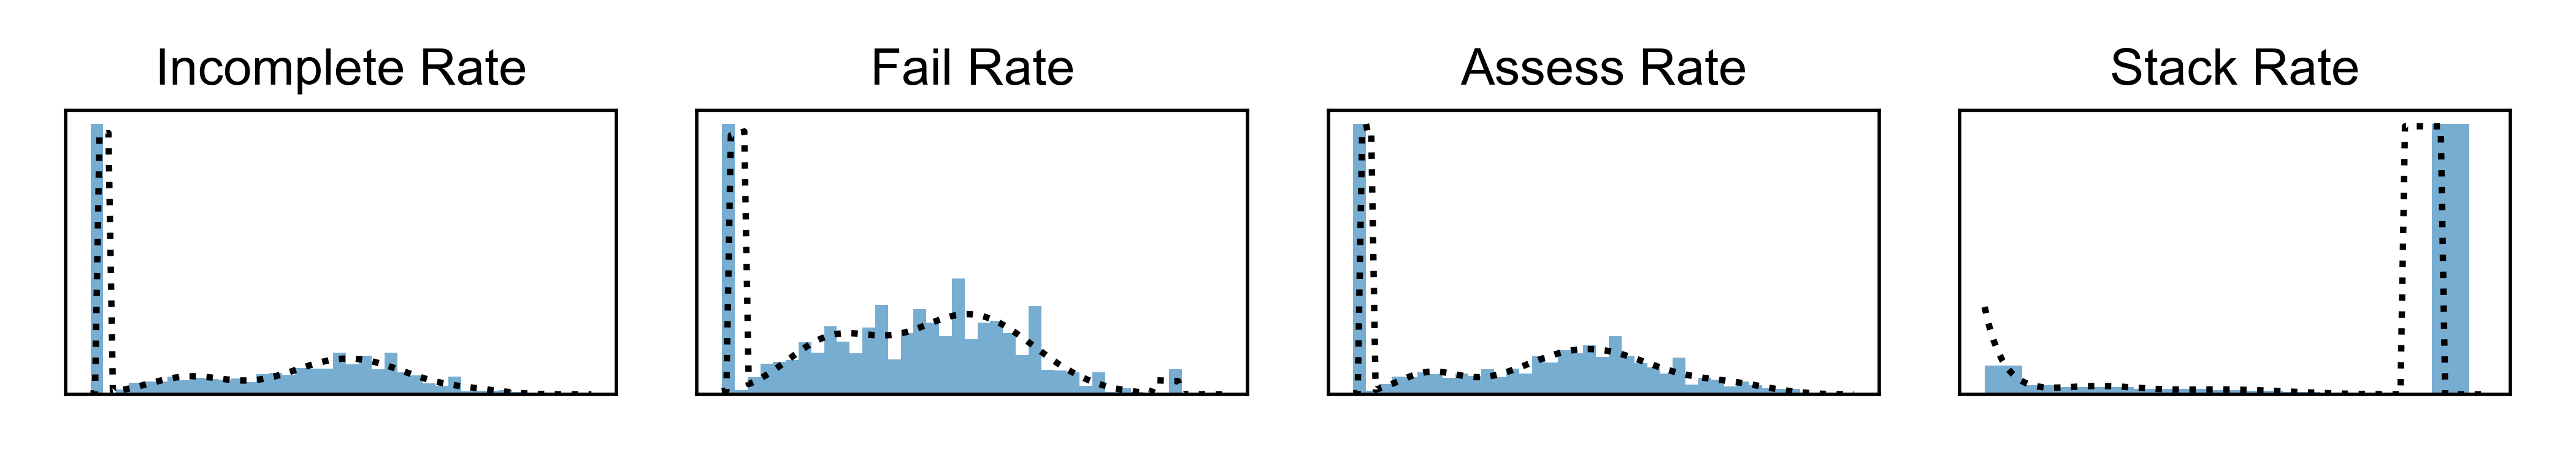
\includegraphics[scale=.6, trim={0 5mm 0 0}, clip]{FittingIndependentFeatures.eps}
\caption{Fitting bespoke mixture model for independent features. }
\label{fig:fitIndependentFeature}
\end{figure}

\vspace*{-3mm}
\subsubsection*{Cluster Churn Rate}
\addcontentsline{toc}{subsection}{Cluster Churn Rate}

We combine the clusters inferred from independent and multivariate features together. For each identified cluster, because we know the churn outcome, we can calculate the proportion of churners, called the \textit{cluster churn rate}. In \Cref{fig:cluster} we show the average cluster size and the associated churn rate. The ``average'' here is the average size for clusters of the same churn rate.

\begin{figure}[htb]
\centering
\vspace*{-3mm}
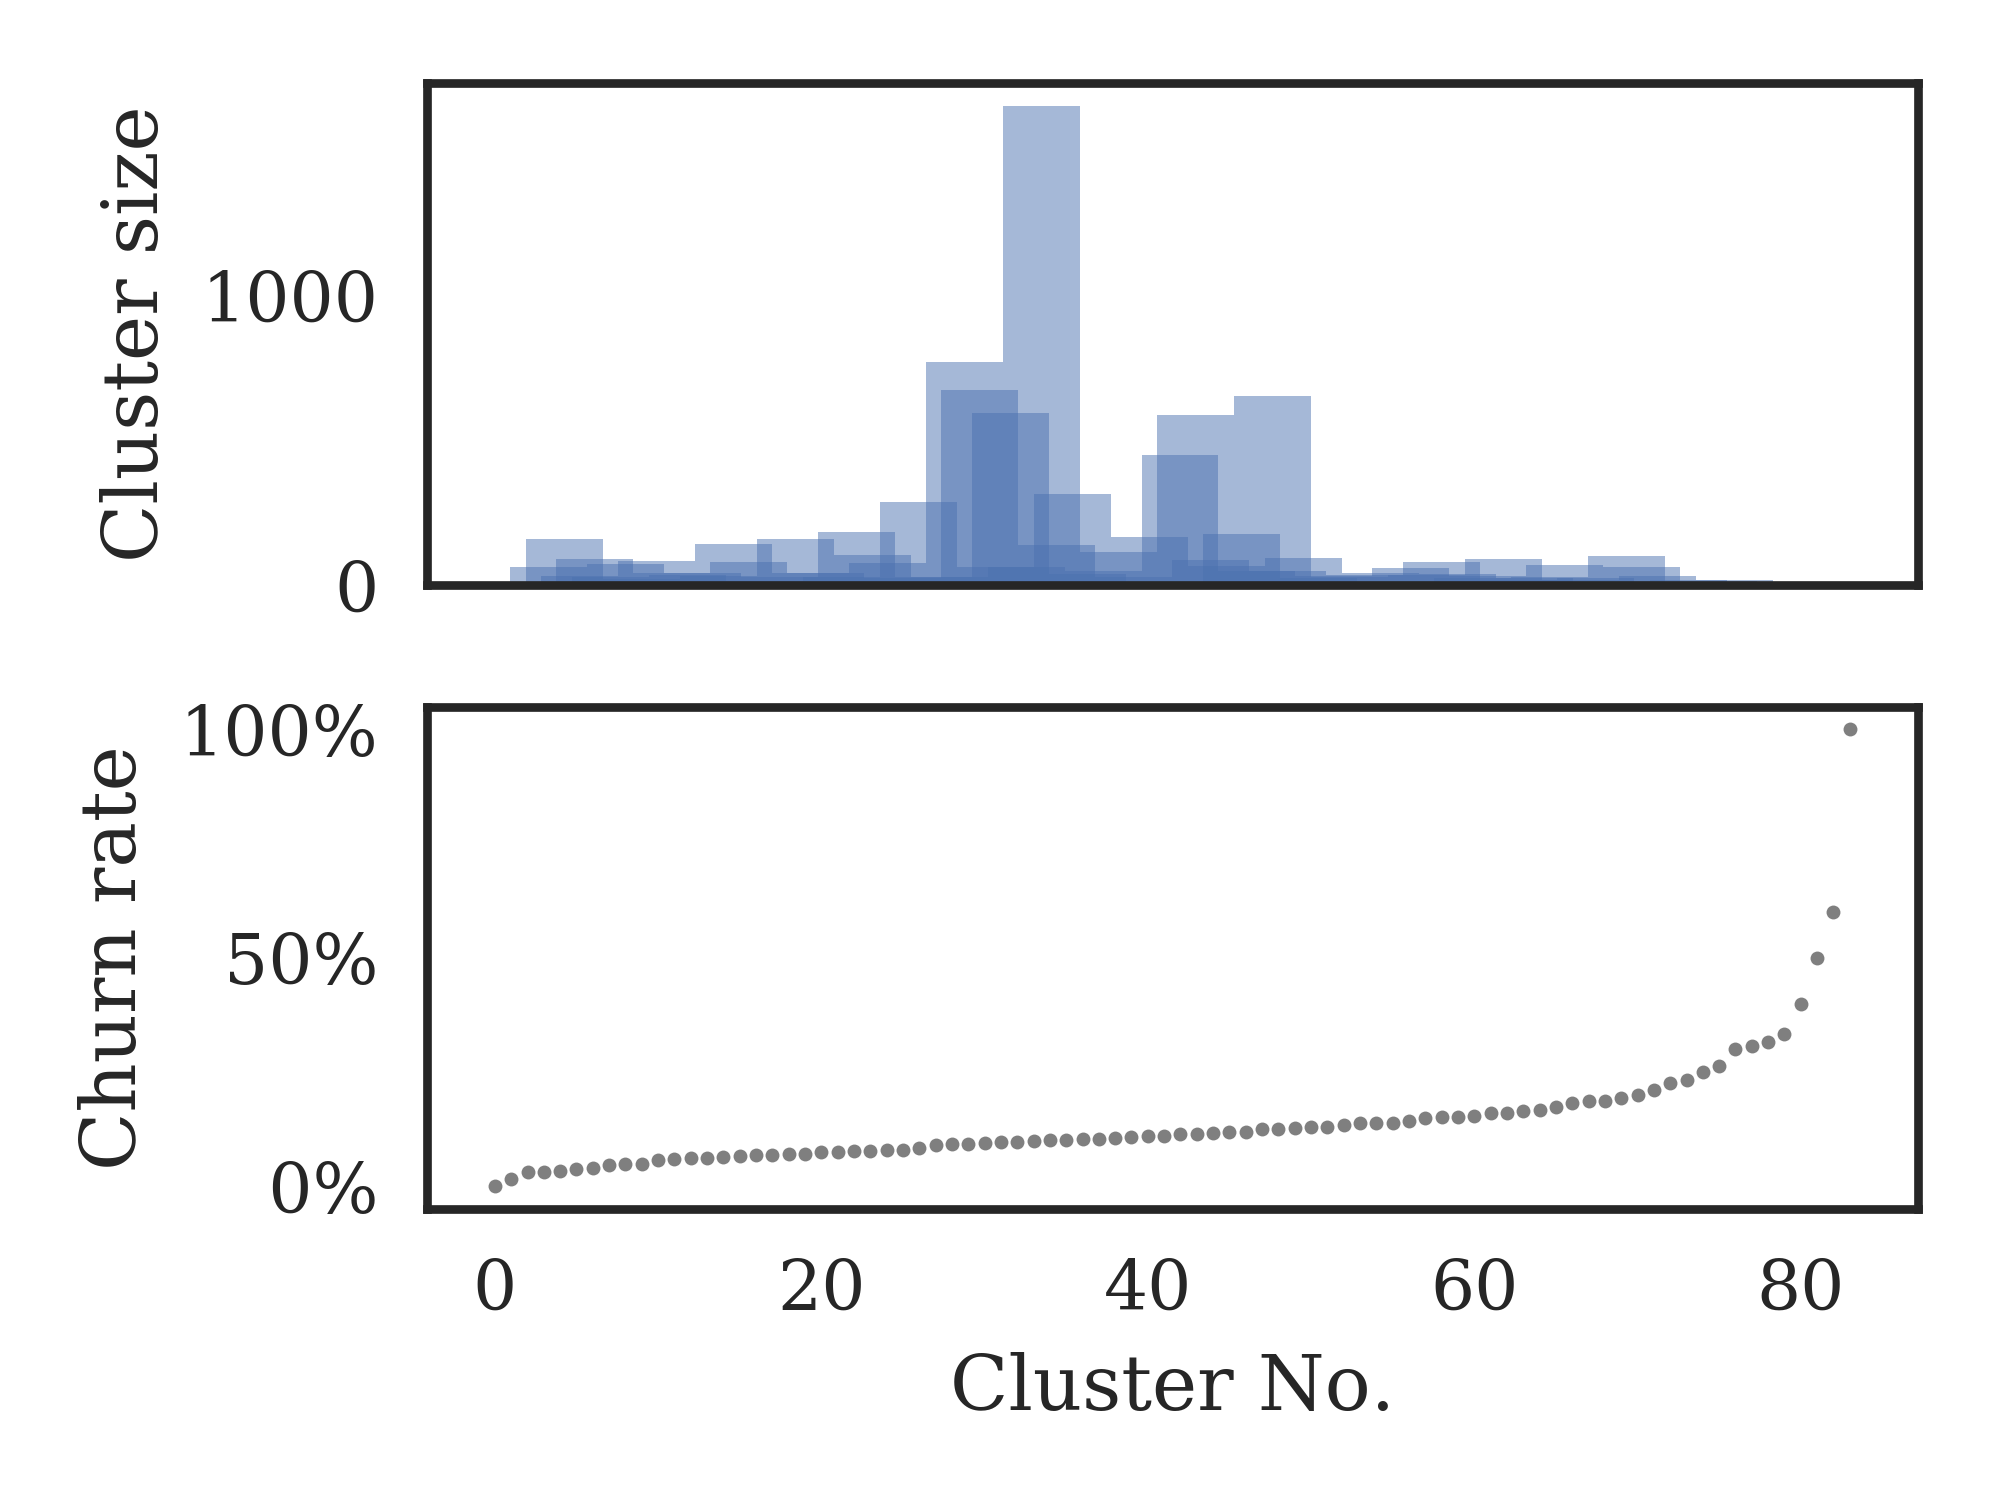
\includegraphics[scale=.6]{ClusteringG3_Complete.eps}
\vspace*{-3mm}
\caption{Identified clusters, their average size and associated churn rate.}
\label{fig:cluster}
\end{figure}

The model identifies a couple of clusters with 100\% and 0\% churn rate. However, the cluster size is really small for these extreme high/low churn rate. This implies that it is much easier to identify ``normal'' customers where the churn probability is around the population average, but really challenging to distinguish ``risky'' or ``safe'' customers who have very high or low chance to churn.

\subsection*{Churn Probability and Markov State}
\addcontentsline{toc}{subsection}{Churn Probability and Markov State}

\infommmarginnote[10em]{The behaviour based model has the predictive power to distinguish pupils with very different churn probabilities!}

Because we have assumed that each pupil has independent behaviours from others, and that customer month are independent in leading to churn outcome, we can interpret the cluster churn rate as the probability of churn of each individual pupil in that cluster. This allows us to have the distribution of individual churn probabilities, shown in left of \Cref{fig:state}.

Looking at the distribution of churn probabilities, we can observe a few concentrations of pupils centered at churn probabilities of approximately 0\%, 12\%, and 25\%. If the behaviour based model did not work at all, the inferred churn probabilities would be purely random, and would converge to a normal distribution due to central limit theorem. Distributions shown in \Cref{fig:state} are definitely not normal. This has shown that the behaviour based model has the predictive power to distinguish pupils with very different churn probabilities. In other words, pupils with the intention to churn exhibit different behaviours than those otherwise.

\begin{figure}[htb]
\vspace*{-3mm}
\centering
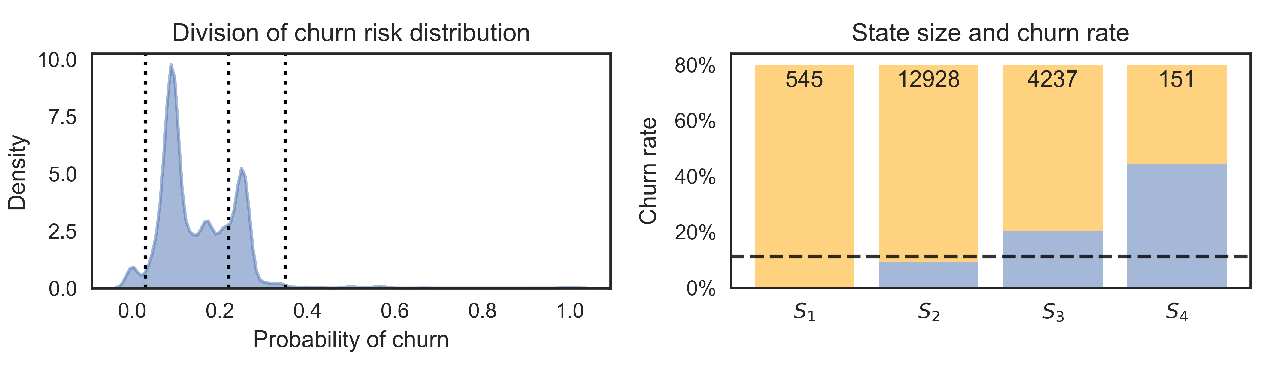
\includegraphics[width=\textwidth, trim={0 5mm 0 0}, clip]{StatesDefinition.pdf}
\caption{Defining Markov states by grouping together pupils of similar levels of churn risk. The right plot shows the size of each state as well as churn rate. The dashed line indicates the level of population churn rate.}
\vspace*{-2mm}
\label{fig:state}
\end{figure}

We define the Markov states by grouping together clusters of similar churn rates because we want the states to indicate churn risk level. In right of \Cref{fig:state} we show an example. We choose to form 4 states $S_1$, $S_2$, $S_3$ and $S_4$ by grouping clusters according to 3 anchor points: 0.3, 0.22, and 0.35 (the three vertical dashed line shown on the left plot). The state churn rates are 0.0\%, 11.7\%, 25.4\% and 55.6\% respectively. Therefore, we can say $S_1$ is the safest state where pupils in this state are very unlikely to churn. In contrast, $S_4$ is a risky state in the sense that pupils in this state are 5.5 times more likely than average to cancel the subscription.

\vspace*{-3mm}
\subsection*{Transitional Analysis}
\addcontentsline{toc}{subsection}{Transitional Analysis}

Following the state definitions in the previous section, we can move to the transitional analysis. We assume stationarity of the Markov chain and estimate the transition probabilities by maximum likelihood. Note that we need to add a state $S_\text{churn}$ that once entered cannot be left (called an absorbing state). Hence, the complete state set is $\{S_1, S_2, S_3, S_4, S_\text{churn}\}$.

The transition probabilities are visualised in \Cref{fig:sankey} as a Sankey diagram. Churned pupils (those in $S_\text{churn}$) cannot transit to other states. $S_2$ is the largest destination state, which makes sense as $S_2$ represents a ``normal'' state in which the churn probability is approximately the same as population average. Very few pupils transit from other states to $S_1$ (the safest state) or $S_4$ (the riskiest state). This seems imply two behavioural paths. First, if a pupil is very likely to stay live in the subscription (in $S_1$), then his intention of exit will be gradually accumulated since most likely he will transit to $S_2$ in the next period and $S_2$ again the next. Second, the reason for strong intention of churn might be purely external and irrelevant to customer experience at Whizz, since there is little chance of transiting to $S_4$.

\infommmarginnote[10em]{State transition probabilities help us understand behaviour dynamics.}

\begin{figure}[htb]
\centering
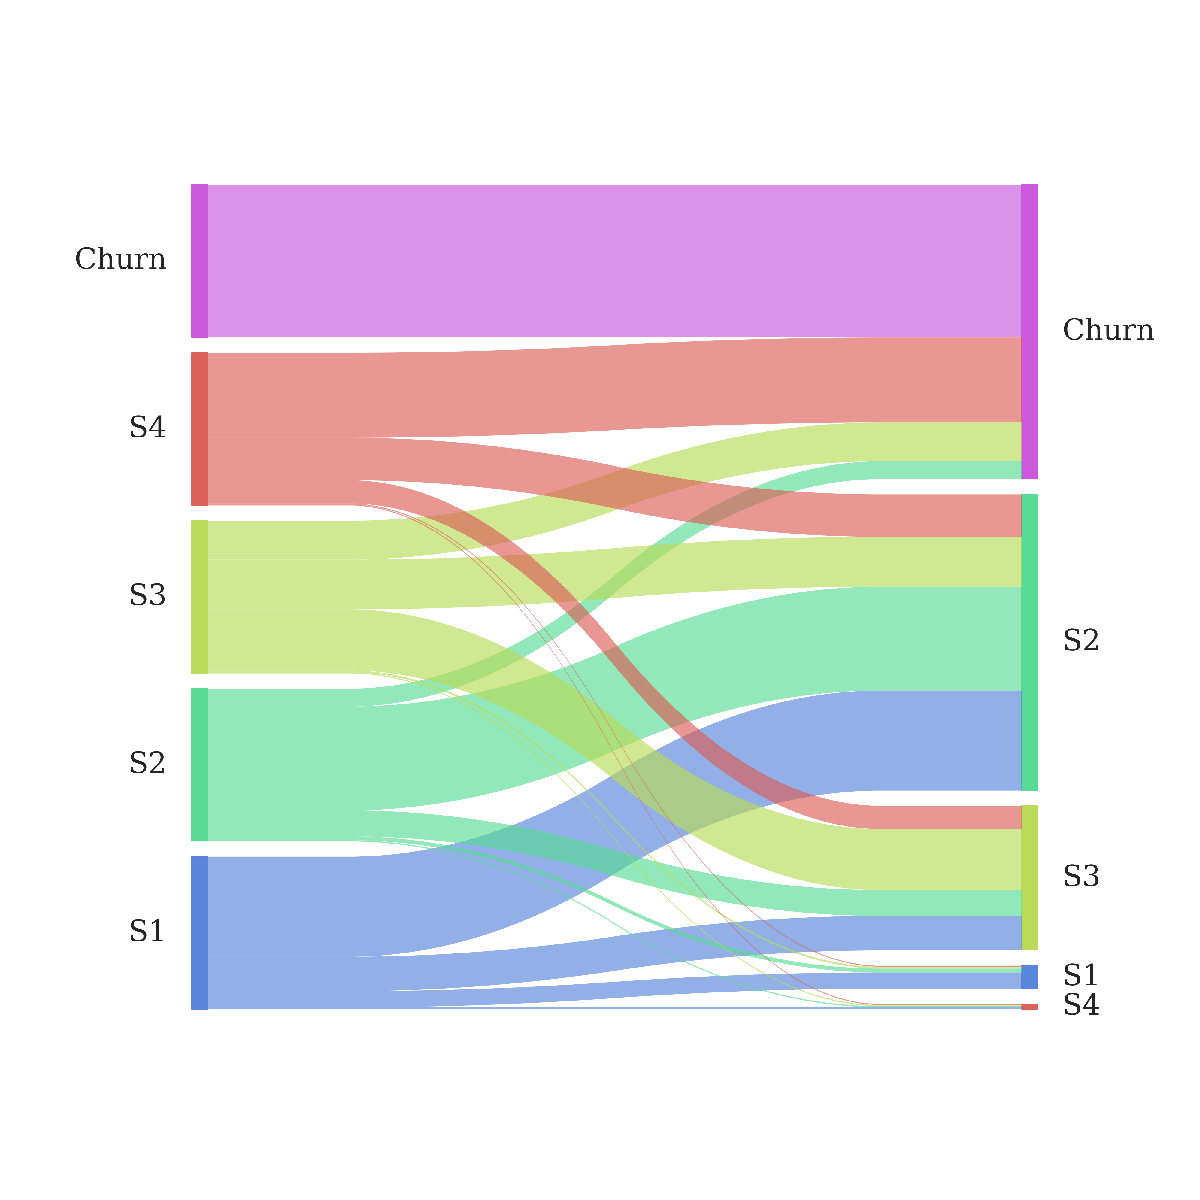
\includegraphics[scale=.38, trim={0 3cm 0 3cm}, clip]{Sankey.pdf}
\caption{Sankey diagram showing the transition probabilities between states. The thickness of each band represents the magnitude of the transition probability from the state on the left to the state on the right.}
\label{fig:sankey}
\end{figure}

\vspace*{-5mm}
\section{Discussion, conclusions \& recommendations}

To help predict churn risk of pupils from the subscription to Whizz online tutorial service, we have proposed a mixture based model which identifies behaviour clusters associated with distinguished levels of churn rate. Moreover, we fitted this model into a Markov chain setting to allow us understand temporal customer behavioural path. The sequential modelling processes have been formulated into a scalable pipeline that can be easily reused, updated and extended.

We described customer behaviours using a state-cluster-observation generative process. The mixture based model infers clusters from observed behaviours, and clusters are grouped to form states by bespoke risk appetite. We have formed 4 states from Whizz's data where the ``riskiest'' state has a churn rate 5.5 time higher then the population average. The model trained from observed data is then used to make prediction on the churn risk of active pupils, and also analyses the potential causes of such risk.

This mixture based behavioural model in churn prediction appeals to be a good approach and there's room for future work. First, we have not discussed in details about the feature selection and feature engineering, though the model itself can absorb any number of features. Selecting independent, informative features may greatly improve the clustering outcome and prediction accuracy. There is room to mine useful information from Whizz's pupils activity database. Second, it is possible to extend the analysis about how feature impacts churn risk. One direction is to find a way to compare feature importance, which translates into measuring importance of dimensions in a multivariate setting. This will be very useful to help the downstream CRM team to prioritise retention strategies.  

Dr. Junaid Mubeen, Director of Education at Whizz Education said: ``\emph{We are very pleased with Victor's contribution. He has addressed our key requirement of developing a model that allows us to predict the likelihood of home users cancelling their subscription from one month to the next. Discussions are already underway with our Development and Marketing teams to understand how we can make use of Victor's model on a continual basis to turn around customers ``at risk'' of cancelling. Victor has also illuminated a number of Machine Learning strategies that we can see having applications in other business problems.}''


% Add the bibliography.
%\begin{small}
%	\nocite{*} % Publishes any unused references.
%\bibliography{references}
%\end{small}
\end{document}